% Author: Animesh Garg
% Date: June 26, 2013

\section{RELATED WORK}
\label{sec:relatedWork}

Grasping and manipulation of real world objects has been studied for over 
a century. The problem of fixturing objects, whether by use of mechanical 
jigs and fixtures, or by actuated robots, has garnered research interest across
disciplines.

A review of Grasping and closure for robotics is provided by 
Bicchi and Kumar \cite{bicchi2000robotic}. A detailed explanatory material 
on grasping has been provided in \cite{prattichizzo2008grasping}. 

As covered in both \cite{bicchi2000robotic, prattichizzo2008grasping}, a 
fundamental requirement of grasping and manipulation is to constraint an object 
in equilibrium and control position and orientation of the object as needed. 
Grasp closure has been characterized in two useful manners: Form Closure and
Force Closure. 

The joint vector of forces and moments at a contact point in $\mathbb{R}^3$ is 
defined as wrench. An rigid object grasped by a set of rigid contact points 
(may be fixed or actuated), is said to be under form closure if it is impossible to 
move the object. Similarly, a rigid object is said to be force closed if an 
arbitrary wrench can be counteracted by a change in contact wrench intensity.
Force closure is similar to form closure but relaxed to allow for friction 
forces to balance object wrenches. 

In applications of fixturing and grasping in healthcare, form closure
is preferred  over force closure due to requirement of a passive positioning systems.  For instance in SRT, a patient's head needs immobilization using a un-actuated device to ensure complete stability while treatment. 

Trinkle \cite{trinkle1992quantitative} provides a quantification of the form closure grasp. Markenscoff et al \cite{markenscoff1990geometry} proved that non-exceptional frictionless object can be grasped in form closure with 
only seven contact points by considering infinitesimal perturbations of the contact points away from the maximal inscribed sphere.Their proof could also be used as basis for algorithms to synthesize form closure grasps. We note that choosing this minimal set of contact points can result in a high normal contact force at a subset of contacts. In medical fixturing, such characteristics of a fixture are undesirable because they may lead to localized pain, skin rupture 
and even injury. Hence we propose the use of surplus contacts for form closure. 

\begin{figure}[t!]
  \begin{center}
    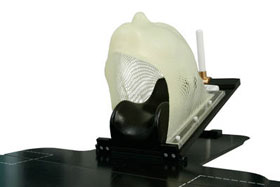
\includegraphics[width=0.75\linewidth]{images/headstep}
  \end{center}
  \vspace{-10pt}
\caption{ The figure shows a Elekta HeadStep used for Stereotactic Radiosurgery.
As illustrated in the picture, the patient head is placed in a frame and secured in place with elastic mask}
  \vspace*{-15pt}
  \label{fig:HeadStep}
\end{figure}

%Related work on grasping with redundant contacts
Modular grasping fixtures have been described by Brost and Goldberg al 
\cite{brost1996complete}. Grasping deformable objects has been a challenge 
in manipulation research. Gopalakrishnan and Goldberg 
\cite{gopalakrishnan2004Dspace} describe new techniques using D-Space for
holding deformable parts. Borst et al \cite{borst1999fast} proposed a 
fast and robust grasp planner. Fast grasp planning and fixturing has since been 
explored by a number of research efforts like Han et al\cite{han2000grasp} who proposed Grasp analysis as linear matrix inequality problems. Liu et al \cite{liu2004complete} describe an efficient algorithm for searching 3-D form-closure grasps in the discrete domain.


Teichmann and Mishra \cite{teichmann2000probabilistic} provided an algorithm for 
grasp quality optimization by a reduction of grasping problem given a set 
of contact points to a convex set cover problem. Ferrari and Canny
\cite{ferrari1992planning} published a seminal work on
geometric grasp quality metrics. They quantified the concepts of total 
force and maximum force as convex hull and minkowsky sum of contact wrenches,
respectively.

Wang \cite{wang2000optimum} proposed an optimal 3D part fixture design 
methodology for a given point set of contact points. 

%Related work on medical fixtures
Bale et al \cite{bale1999new} propose a new vaccum based device for
extremity immobilization. 


Labadie et al \cite{labadie2009customized} introduced a micro stereotactic table for surgery with a degree of customization.Brown et al\cite{brown2002application} explored use of stereolithography for orthopedia treatments.\cite{fitzpatrick2005accuracy} studies the accuracy of customized 
stereotactic platforms.
%List commeercial stuff from Elekta
There are a number of commercial medical patient positioning systems currently
used in clinic. As shown in figure~\ref{fig:leskellFrame}, the Leskell coordinate frame G four tapping screws
keep the frame attached to the patient's head. This frame requires local 
anesthesia to minimize patient discomfort during the procedure. 

Figure~\ref{fig:HeadStep} shows a Elekta HeadStep which is used for
immobilization in cranial as well as head, neck and shoulder procedures.
It uses an elastic mask to cover the face and the head with incisions for 
breathing. Figure~\ref{fig:HeadFix} shows a Elekta HeadFix which is used for
head immobilization. A vacuum activated head frame system hold a mouthpiece
to clamp down the patients upper jaw. Customization is in the sense that the impression of the upper jaw is patient specific. 


\begin{figure}[t!]
  \begin{center}
    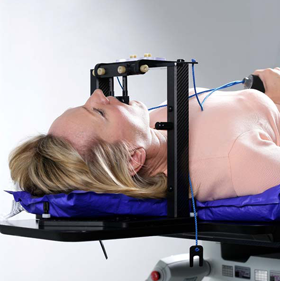
\includegraphics[width=0.9\linewidth]{images/headfix}
  \end{center}
  \vspace{-10pt}
\caption{ The figure shows a Elekta HeadFix used for Stereotactic Radiosurgery.
As illustrated in the picture, the patient head is placed in a frame and secured in place with vacuum activated mouthpiece holding the patients upper jaw.}
  \vspace*{-15pt}
  \label{fig:HeadFix}
\end{figure}


Furthremore, there are several patents on customized surgical fixturing, \cite{franklin2001customized} and frameless stereotactic guidance \cite{bova2010frameless}

Our work extends the findings of Schulman et al\cite{schulman2011grasping}
to applications in medical fixturing. Furthermore we also propose a method of 
initial generation of candidate contact points using geometric intuitions from 
local curvature and also no-go zones as specified by a phycisian (viz. mouth, eyes, ears, nose etc.) 

%Similar methods can also be used for generating form/force
%closure grasps for physical objects using multi-fingered hands or multiple hands. 

%Elekta Leskell coordinate frame G requires anaesthetics to minmize patient discomfort.
%Fixing the frame to the patient’s head is simplicity itself - four self-tapping 
%screws keep the lightweight frame firmly and accurately in place, while local 
%anesthesia minimizes any patient discomfort during the procedure.

%Elekta HeadSTEP
%Its excellent robustness and quality guarantees precise and simple 
%repositioning in routine cranial as well as head, neck and shoulder 
%immobilization.